\section{Object oriented transients and steady state}

The greatest strength of object-oriented programming is also directly related to the greatest source of poor and inflexible
designs. Polymorphism allows one to separate interface from implementation making it possible for an object to depend
on an abstraction instead of a concrete implementation. In theory, we can plug one of several possible implementations
into an object at runtime. 

In steady-state, when the program can be seen as a graph of communicating objects, this scheme works very well. The
problem is the initial construction of this graph which is when a concrete implementation must be selected for
each object reference. In terms of program control flow, there are only two ways of filling in an abstract reference:
internally or externally.

Internal control flow is when the configuration of a reference is initiated by a method of the same object that holds
this reference, for example its constructor method. The easiest and most commonly used way to fill the reference is
to simply create a new instance of a concrete implementation class. The problem, of course, is that now the client
class is tied to a specific implementation and we can no longer plug in alternative implementations, negating the
benefits of polymorphism. Direct instantiation also has a direct influence on physical dependencies. The client
class' module now depends directly on the module containing the implementation class.

The problem here is that there is no such thing as a polymorphic constructor. With internal control flow
the only way to decouple a class from a specific implementation class is to delegate the creation of objects.
Several of the Creational Patterns \cite{Gamma} are ways of implementing this delegation, the most commonly
used being the Factory Pattern. A factory is an object whose purpose is to encapsulate the instantiation of
other objects. A client object can fill in an abstract reference without being tied to any concrete implementation
using a factory object. However, this pattern simply trades the coupling to one concrete class for the coupling to
a specific factory class.

A difficulty with the factory pattern is the obtention of a reference to a factory object. Direct instantiation is
not commonly used because this restricts the flexibility of the factory implementation too much. A widely
used scheme is to use the singleton pattern to ensure that there is only one, globally-visible instance of the
factory. This has the advantage that the creation of objects is consistent for all clients because there is only
one configuration of the factory. The drawback is that all clients are tied to a concrete factory class on a logical
and physical level. In addition, it is cumbersome to supply different implementations of the factory to
create \emph{mock} objects for testing purposes. Another possibility is to pass a reference to a factory object
to the constructor method, which allows to split the factory into interface and implementation and to have several
instances. This simplifies testing because a different factory implementation can be supplied for testing purposes.

The flexibility of the externally supplied abstract factory leads us to the external configuration control flow:
all abstract references of an object could be supplied externally either as arguments to the constructor method
or during a special initialization phase. Following this approach the object's method are written assuming a
steady-state situation, the concern of dependency resolution is left for an external party to resolve. This has
many benefits because the object can depend only on abstract interface classes. To put it in a different way, the
functionality is now performed entirely in terms of abstract operations. This reduced coupling is beneficial for
software maintenance because the implementations of the other objects can evolve without affecting this client
object. It also facilitates testing because \emph{mock} object can be supplied. In terms of physical design
the only dependencies left are the dependencies on the modules containing the interface classes.

The same discussion applies to software components, as they can be seen as coarse-grained objects at runtime. Many
component frameworks such as COM, EJB or CCM expect an internal control flow for the configuration of components.
A basic service offered by these platforms is a global directory or a registry. Every component can register
itself using a symbolic name. To find other services it depends on, a component uses a shared symbolic name
to look it up in the registry. In a way, a global directory service is just another manifestation of the factory
pattern with a singleton implementation. Therefore, although components are decoupled from each other, every component
is strongly tied to the platform infrastructure with obvious drawbacks such as the lack of portability and independent
deployment. The deployment of such a component always requires the deployment of the the framework modules.
To make matters worse, these platforms often require components to implement one or more standard interfaces.
Inheritance, be it of interface or implementation, is the strongest coupling in an object-oriented programming language
and therefore even components without external dependencies cannot easily ported to other frameworks.

In addition to dependencies on other components, components also often support parameters for their execution
that must be configured. Most of the times these parameters are not hard-coded but left open for configuration
during initialization. With internal control flow there is no way of retrieving the values for these parameters
without making many assumptions about the execution environment. A component framework could have a registry
for configuration values or the component could read a configuration file. But in all cases it depends on
a significant infrastructure to do so.

An amusing way to see internal configuration control flow appears if we extend the analogy between software components
and electronic components: electronic components searching for each other on the circuit board instead of just assuming
they are correctly connected.

\section{Dependency injection frameworks}

The lack of portability and interoperability between components developed for different frameworks, among other reasons \cite{Dearle},
has lead the development of so-called \emph{lightweight containers} such as Spring, PicoContainer and Guice \cite{Spring},
\cite{PicoContainer}, \cite{Guice}. These containers are based on an idea called \emph{dependency injection} \cite{Fowler2}.

Dependency injection is often called \emph{inversion of control}, but but it is really only a special case \cite{Fowler1}.
Inversion of control happens when a programming framework calls the application code instead of the other way around.
For example, in windowing frameworks, when the user captures a button, the framework calls the application code.
In contrast, in a command-line program it is the application code that initiates a request to read data from the standard input.
Arguably, inversion of control is a defining features of frameworks, separating them from mere libraries.

Dependency injection involves the inversion of control flow during the configuration of an object or component.
The idea is that there is a special layer in the application that is responsible for the composition and configuration
of application components \cite{Sobernig}.

What separates manual external configuration and dependency injection are generality and physical dependencies.
A piece of manual configuration code contains a lot of repetitive code for the instantiation and connection
of objects and is therefore hard to maintain because of issues such as the order of instantiations. In addition,
because it uses direct type definitions, there is a direct physical dependency on other module. Otherwise,
a dependency injection procedure takes a declarative representation of the connected object graph
and returns the desired graph of objects. All the code for the ordering of instantiations and connections
is generic and reusable. Of course, for this to be possible it must be possible to handle classes and objects
of unknown types. A direct consequence is that the dependency injection code is free of dependencies on
the classes it instantiates and can be packaged as a generic library and independently reused.

A crucial requirement for the implementation of dependency injection is the support for a generic and opaque
handling of classes and objects that removes any compile-time or link-time dependencies. Runtime reflection
as supported by a meta-object protocol \cite{Kiczales} or even a pure runtime type introspection such
as built in the Java language is the most common enabler of dependency injection. Aspect-oriented programming
has also been proposed as an implementation tool for dependency injection as it has reflective capabilities
\cite{Chiba2005}.

Dependency injection usually comes in three flavors: constructor injection, attribute injection and setter injection.
Constructor injection is when references and values are passed to an object as actual parameters to its constructor.
Constructor injection guarantees that an object is never in a inconsistent state between construction and initialization
but makes object circles impossible. Attribute injection happens when the public attributes of an object are modified
directly. Setter injection, happens when accessor methods, are used to change the value of an attribute. These last
two forms are more flexible but create a state when the object is already created but not ready to run. For this reason
dependency injection frameworks that support attribute or setter injection usually also support initializer methods
without arguments that are called when the configuration phase is finished.

Different dependency injection frameworks also differ in the declarative representation of the configured object graph.
The most popular approach, implemented by Spring, is to define an XML configuration language. This input is then
kept as a separate configuration file and allows rewiring the object graph without recompilation. The drawback
is that this configuration is invisible to code refactoring tools present in development environments such as eclipse.
If such a tool is used on a large code-base, many changes must be reflected manually on the configuration file and
errors are only discovered during execution. For this reason, Guice keeps this configuration information as Java code.
Guice makes extensive use of Java annotations to mark attributes that must be configured, identify initializer methods
and so on. Java annotations have the advantage that they don't introduce hard dependencies between modules.
A module with Guice annotations can be deployed and used without any Guice module.

Due to the requirement of introspection dependency injection frameworks are usually only available for languages
that support it, such as Java. There is, however, a framework for C++, PocoCapsule that does a limited form of
dependency injection \cite{PocoCapsule}. This framework has a tool that takes as input a configuration file and
the header files containing the class definitions and generates code for the instantiation and configuration
of objects, but only for the constructors, attributes, and acessor methods explictluy mentioned in the configuration
file. This approach allows to make small changes to the configuration file such as the change of parameter values
but more extensive changes in configuration require recompilation.

A popular feature of dependency injection frameworks for Java is \emph{auto-wiring}. The Java community has a
long tradition of using standard naming schemes for classes, attributes and methods that makes it possible to
use introspection for inversion of control, an approach called convention over configuration. For example,
acessor methods for a variable called \texttt{foo} are always spelled \texttt{setFoo} and \texttt{getFoo}.
Dependency injection frameworks such as Spring require that a name is given to identify each object. When
auto-wiring is enabled, any object whose name happens to be \texttt{foo} is injected in every other object
that has a public attribute called \texttt{foo} or a \texttt{setFoo} setter method.

The link between dependency injection and feature-based programming of product lines has not passed unnoticed.
Walraven \emph{et al.} proposed the use of dependency injection to enable multi-tenancy in Software-as-a-Service
(SaaS) applications \cite{Walraven} \cite{Truyen}. In their approach service is offered with some feature variations.
To each customer, or tenant, a specific composition configuration is associated and is applied using dependency
injection. Rosa and Lucena Jr. also propose the use of dependency injection to automatically configure a mobile
application according to the execution platform \cite{Rosa}.

Dependency injection has already been used to separate the concern of the communication protocol used between
service components, but this is the subject of chapter \ref{chap:sca} and will be discussed in more detail there.

\section{The benefits of dependency injection}

Dependency injection as opposed to what Fowler calls the \emph{Service Locator Pattern} has many benefits.
It is an effective tool for the realization of several of Knoernschild's modularity patterns. It provides
a common framework for the \texttt{External Configuration} pattern. It makes the \textbf{Container Independence}
pattern possible without requiring the application programmer to write an insulation layer. It also greatly
aides the \textbf{Abstract Module} pattern together with the closely related \textbf{Separate Abstractions} pattern
by providing a non-intrusive way of injection concrete implementations into abstract reference.
Dependency injection, short D.I. also impacts many other aspects.

\textbf{Maintainability} D.I. aides the reduction of coupling because it effectively support interface-based
design. But this does not mean that it enforces this design. It is possible to create tightly coupled
designs on top of D.I., although it is probably easier to refactor such a design to an interface-based
one because the hardest part, the assignement of the responsibility to select implementation, is already
done. In a sample of open-source projects, Razina and Janzen found no significant correlation between
measures of cohesion and coupling and the use or not of D.I. However, among the projects that used D.I.
they observed a trend to lower coupling in projects that made a more extensive use of D.I. \cite{Razina}

\textbf{Reuse} By enabling container independence and abstract dependencies, this approach makes component
code more reusable because it can be used in many situation without modifications. With D.I the same
component can be reused across many different platforms. Because the core functionality is separated, it
is easy to write adapters, if necessary, for containers that rely on service locators. It can also be
used without any container at all. The converse is also true. Pre-existing objects can be used in a
D.I. container without modification.

\textbf{Physical design} When components are designed to use a service locator, a dependency is created on its API
that manifests itself at the physical layer. The component module is now has a dependency an the module that
contains the API definition.  With D.I. this dependency is eliminated and the component module can be
deployed independently of any infrastructure module.

\textbf{Intentionality} Intentionality is a subjective code measure that captures to what degree it is possible to
understand the specification of a piece of code only by reading it. It is defined by Armstrong as follows \cite{Armstrong}:

\begin{quotation}
``Intentional Programming - this is a programming style where the programmer can easily see from the code exactly
what the programmer intended, rather than by guessing at the meaning from a superficial analysis of code''
\end{quotation}

Another definition is given by Czarnecki \cite{Czarnecki98}:

\begin{quotation}
``... decrease the conceptual gap between program code and domain concepts (known as achieving high intentionality)...''
\end{quotation}

We say that intentionality is subjective because it is influenced by a several factors such as the familiarity of
the reader with the programming language and libraries being used and the overall structure of the code. Despite
this subjectivity it should be clear that if a piece of code is cluttered with secondary concerns it will be
less understandable and therefore have a lower intentionality. This has to do with the principle of separation of
concerns as is explained very lucidly by Czarnecki:

\begin{quotation}
One of the most important principles of engineering is the principle of separation of concerns.
The principle acknowledges that we cannot deal with many issues at one, but rather with one at a
time. It also states that important issues should be represented in programs intentionally (explicitly, declaratively)
and well localized. This facilitates understandability, adaptability, reusability, and the many other good qualities 
of a program since intentionality and localization allow us to easily verify how a program implements our requirements.
\end{quotation}

We claim that dependency injection increases the intentionality of code because the concern of locating external
components is separated from the task that a piece of code is written to accomplish. Also the dependency on external
components is explicitly represented in the external representation of a concrete class. For example in Java
references are represented as attributes or pairs of accessor methods and are subject to introspection.

Also, as will be discussed more thoroughly in the chapter about \texttt{SCA}, dependency injection has the potential
to remove direct code dependencies on the component framework being used and which further helps to simplify the
code.

\textbf{Portability} In many situations programming frameworks act as factories or service locators. For example
components built on top of CCM explicitly call the CCM framework to locate other components. This means that CCM
components are tightly coupled to the CCM runtime and cannot be reused in other situations. In other words, they
are not portable. In contrast, if we look at applications developed using the Spring Framework for Java we will
see that they are POJOs that never reference Spring's API and can therefore be used in other contexts.

\begin{center}
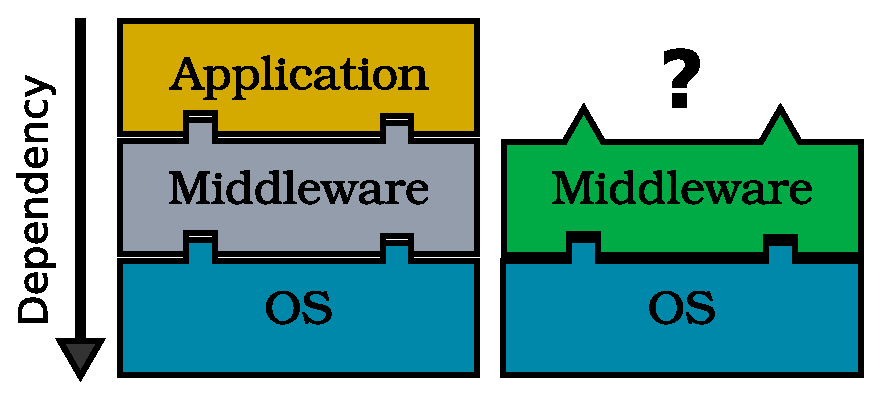
\includegraphics[height=80pt]{graphics_tables/bad_layers.eps} 
\end{center}

The problem with the earlier component framework is that they are based on a strictly layered approach. Traditionally systems
are structured in layers where the more abstract layers depend on more the concrete layers below them. The benefit is that
the higher level layers can be built without worrying about low-level concerns. The drawback is that the higher level
layers are tightly coupled to the layers directly below them and are usually not portable to other stacks.
This problem can be mitigated by creating standards for the API of a layer, like \texttt{POSIX}, but cannot be completely
eliminated. 

With inversion of control, the infra-structure can sometimes be abstracted away completely eliminating source dependencies
on infra-structure APIs. As will be explained in the chapter about \texttt{SCA}, dependency injection can be used to adapt
a generic component to a specific middleware platform.

\begin{center}
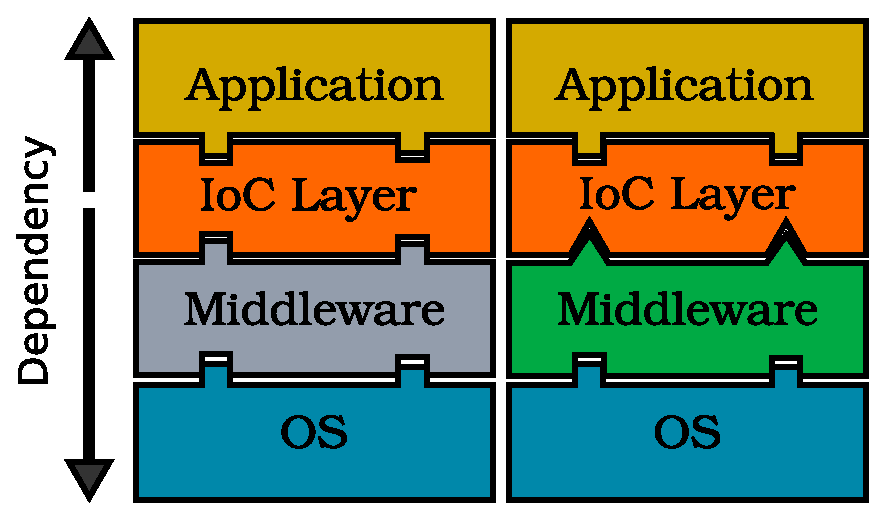
\includegraphics[height=80pt]{graphics_tables/good_layers.eps} 
\end{center}


\textbf{Interoperability} Component frameworks like CCM are created to foster the reuse of software components.
Unfortunately these component frameworks are incompatible: a component in a CCM container cannot use a COM
component directly. So the platforms created to enable reuse can actually hinder it in some situations, creating
islands of compatibility. 

There are several solutions to bridge the gap between different middleware platforms such as the translation of
network protocols. But it would be even better if the component framework to use was just a matter of external
configuration. Then we could take two components and configure the remote method invocation protocol they should
use to talk to each other.
